
\begin{figure}
\begin{center}
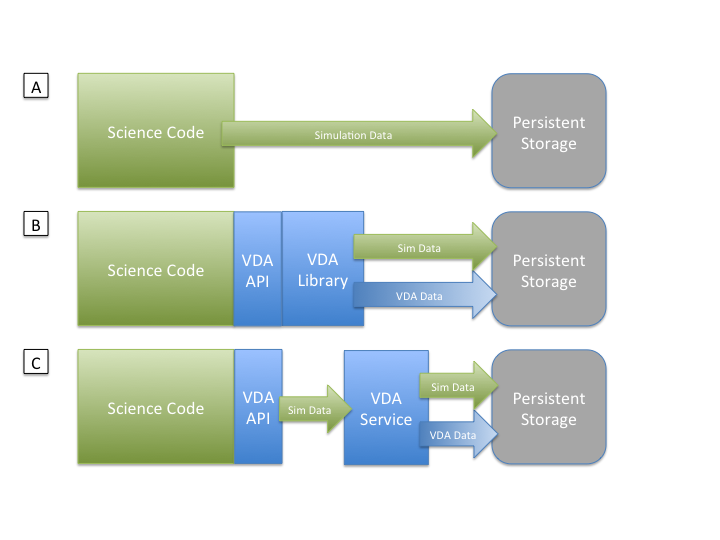
\includegraphics[width=6in]{figures/three-data-flows}
\end{center}
\caption{ A simplified pipeline diagram showing the flow of information from simulation to persistent storage in one example of a modeling and simulation workflow (we note that writing to persistent storage is not the only end state of analysis, as is explained WHERE).  Most data analysis today occurs as a \emph{post-processing} step, as in pipeline \textbf{A}.  However, as we move to extreme scale science, we must adopt workflows that integrate VDA more closely, either as in pipeline \textbf{B}, as a library compiled into the simulation code, or as in pipeline \textbf{C}, as a loosely coupled service.  In either case, we expect a standard VDA API to be used by the science code, so that VDA code can be executed efficiently according to the hardware and execution policy available.
\label{simplepipeline}}
\end{figure}

Why is science at Extreme Scale so different from current practice?  Can't we
continue using the successfully deployed applications for this new scale, if, like science codes, we adapt to the challenges of the new architectures?

The answer is, simply, no.  A major challenge moving from current architectures to extreme architectures and extreme scales are twofold.  First, the rate of 
computation far outstrips the rate of I/O for a large system.  Second, it is
prohibitively expensive in terms of power to move large datasets from memory,
across networks, to disks.  These two considerations, spelled out in detail in
HERE HERE and HERE, require us to alter our current analysis pipeline.

More importantly, there are system wide implications resulting from the solution
to this problem, which include domain and technique specifc analysis techniques,
in-situ framework development, and complexity impacts in post-processing.

Figure~\ref{simplepipeline} shows simplified diagrams showing the flow of information from simulation to persistent storage in a typical modeling and simulation workflow.  Typical Visualization and Data Analysis (VDA) occurs as a 'post processing' step, after the simulation has written results directly to persistent storage.  Typically, these results are in a code-specific format, and are formatted as 'restart' files - optimized for reading back into an instance of the science code, and not optimized for post processing analysis by VDA tools.  Extreme computation size and extreme architectures force data flows like (b) and (c), in which VDA is performed on the simulation results before they are written to persistent storage.  In (b), data is handed directly to a VDA library coupled with the running code.  In (c), data are 'sent' to VDA process separate from the running code, enabling analysis, visualization and data reduction under the control of the science code - at the cost of sharing runtime resources with the VDA execution.  This decouples the data computation and VDA processes, which affords many advantages, at the cost of system complexity.  Both approaches must be provided for extreme scale analysis, so that the codes, system designers, and science customers can design a computation and analysis workflow suited to the specific needs of the science, analysis and decision support being supported.
